\documentclass{article}


% if you need to pass options to natbib, use, e.g.:
%     \PassOptionsToPackage{numbers, compress}{natbib}
% before loading neurips_2022


% ready for submission
\usepackage[final]{neurips_2022}


% to compile a preprint version, e.g., for submission to arXiv, add add the
% [preprint] option:
%     \usepackage[preprint]{neurips_2022}


% to compile a camera-ready version, add the [final] option, e.g.:
%     \usepackage[final]{neurips_2022}


% to avoid loading the natbib package, add option nonatbib:
%    \usepackage[nonatbib]{neurips_2022}


\usepackage[utf8]{inputenc} % allow utf-8 input
\usepackage[T1]{fontenc}    % use 8-bit T1 fonts
\usepackage{hyperref}       % hyperlinks
\usepackage{url}            % simple URL typesetting
\usepackage{booktabs}       % professional-quality tables
\usepackage{amsfonts}       % blackboard math symbols
\usepackage{nicefrac}       % compact symbols for 1/2, etc.
\usepackage{microtype}      % microtypography
\usepackage{xcolor}         % colors
\usepackage{graphicx}
\usepackage{float}
\usepackage{amsmath}


\title{Exploring Data Cleaning using Language Model for Sentiment Analysis}


% The \author macro works with any number of authors. There are two commands
% used to separate the names and addresses of multiple authors: \And and \AND.
%
% Using \And between authors leaves it to LaTeX to determine where to break the
% lines. Using \AND forces a line break at that point. So, if LaTeX puts 3 of 4
% authors names on the first line, and the last on the second line, try using
% \AND instead of \And before the third author name.


\author{
  Puttisan Mukneam \\
  Pitzer College\\
  Claremont, CA 91786 \\
  \texttt{nmukneam@students.pitzer.edu}
}

\setcounter{secnumdepth}{4}
\begin{document}


\maketitle


\begin{abstract}
In the realm of sentiment analysis, data cleaning is an indispensable but challenging task. This study investigated the potential of applying pre-trained language models to perform data cleaning tasks, specifically in the context of sentiment analysis of Steam reviews. We utilized a suite of models, including gpt2, gpt2-xl, t5-base, t5-xl, and two variations of the recently released flan-t5 model, flan-t5-base and flan-t5-xl. The reviews generated by these pre-trained models were then subjected to sentiment classification using Multinomial Naive Bayes and Support Vector Machines classifiers, and the performance was assessed using Mean Squared Error (MSE), Accuracy, and F1-score. The results varied with the baseline method displaying superior performance. However, the flan-t5-base model showed promising results, with an MSE of 0.96, an accuracy of 75.87\%, and an F1-score of 0.821 when evaluated using SVM. Our project reveals the potential of pre-trained language models in automating and enhancing data cleaning tasks, while also suggesting that more extensive fine-tuning and larger datasets could lead to further improvement.
\end{abstract}

\section{Data Cleaning}
Data cleaning, also known as data cleansing or data scrubbing, refers to the process of identifying and rectifying or removing errors, inaccuracies, and inconsistencies in datasets. This vital stage in the data preprocessing pipeline enhances the quality of data and significantly influences the outcome of the subsequent analysis.

Data cleaning involves several crucial steps. These include removing duplicates, handling missing values, correcting inconsistencies, and dealing with outliers. By ensuring that the data is accurate, complete, consistent, and relevant, data cleaning facilitates the data mining process and helps in making the most out of the collected data.

In the context of sentiment analysis, data cleaning plays a pivotal role. Sentiment analysis, also known as opinion mining, involves interpreting and classifying emotions (positive, negative, and neutral) within text data using text analysis techniques. This process allows organizations to understand the social sentiment of their brand, product, or service while monitoring online conversations.

However, raw data collected from various sources, like social media platforms, reviews, forums, and more, is typically unstructured and often contains noise in the form of irrelevant information, typos, slang, emojis, and so forth. Data cleaning in sentiment analysis is therefore necessary for the following reasons:

\begin{itemize}
    \item \textbf{Noise Reduction}
Raw text data contains a lot of noise such as irrelevant symbols, numbers, punctuation marks, and special characters that may not contribute to sentiment analysis. Data cleaning can help remove this noise, making the data more manageable and the subsequent analysis more accurate.

\item \textbf{Standardization}
Data from different sources can be in different formats or languages, and the same sentiment can be expressed in various ways. Data cleaning aids in standardizing the data, making it possible for the sentiment analysis algorithm to correctly interpret the sentiments.
\item  \textbf{Reducing Dimensionality}
Text data tends to be high-dimensional due to the large number of unique words (known as the vocabulary). This can make sentiment analysis computationally expensive. Data cleaning techniques such as stemming, lemmatization, and stop-word removal can reduce the dimensionality of the text data, making the analysis process more efficient.

\item  \textbf{Handling Missing or Incomplete Data}
Sometimes, the collected data may have missing or incomplete information, which can lead to incorrect analysis if not handled properly. Data cleaning helps in dealing with such issues either by filling the missing values with appropriate techniques or by excluding such instances after careful consideration.

\item \textbf{Improving Model Performance}
Clean and high-quality data is key to the performance of sentiment analysis models. Unprocessed or dirty data can mislead the training process of the models, leading to poor performance. Through data cleaning, the data fed into the models is more representative, leading to more reliable and robust models.
\end{itemize}

\subsection{Data Cleaning in ML task}

The paper "CleanML: A Study for Evaluating the Impact of Data Cleaning on ML Classification Tasks" by Peng Li, and others (2021) makes several important observations that underscore the importance of cleaning data before it is utilized for machine learning tasks [9]. Here are their findings:

\begin{itemize}

\item \textbf{Missing Values}: The paper shows that the imputation of missing values, rather than their deletion, is more likely to improve or maintain the performance of machine learning models. This is a significant observation because missing data is a common problem in datasets. The authors further emphasize that the choice of imputation method and model can increase the positive impact and reduce any negative consequences of this data cleaning step.

\item \textbf{Outliers}: Cleaning outliers seems to have an insignificant impact on model performance. However, the authors note that the choice of model and cleaning algorithm can reduce the probability of negative impacts, emphasizing the importance of strategic decision-making in data cleaning processes.

\item \textbf{Mislabels}: The paper's findings suggest that cleaning mislabels is likely to have a positive or, at worst, insignificant impact on ML. Once again, the choice of model can increase the likelihood of positive impacts, underscoring the need for careful model selection.

\item  \textbf{Inconsistencies}: Cleaning inconsistencies, according to the findings, is more likely to have an insignificant impact and is unlikely to negatively impact ML. This suggests that tackling inconsistencies in the data, while not always hugely impactful, is generally a safe cleaning step to undertake.

\item \textbf{Duplicates}: Cleaning duplicates is likely to have an insignificant or even negative impact on ML. This impact varies across detection methods and datasets, pointing to the importance of understanding the specific dataset and detection method used when cleaning duplicates.

The study reveals that data cleaning - when done strategically and methodically - can be beneficial for machine learning models. Different types of data errors require different cleaning methods, and the choice of model and cleaning algorithm can significantly influence the outcomes. It also demonstrates that while some cleaning steps may not always significantly improve model performance, they rarely harm it, suggesting that a thorough data cleaning process is an important part of the machine learning pipeline. This paper thus provides strong evidence in favor of data cleaning as a good practice in ML tasks.


\end{itemize}


\section{Backgrounds}


\subsection{Language Model}

A Language Model (LM) is a type of statistical model that is used for predicting the next word in a sentence given the previous words. It is a fundamental concept in the field of natural language processing and has applications in various tasks such as machine translation, speech recognition, part-of-speech tagging, and sentiment analysis, among others.

Formally, given a sequence of words $w = w_1, w_2, ..., w_n$, a language model assigns a probability $P(w)$ to the entire sequence, which can be factorized as:

\begin{equation}
P(w) = \prod_{i=1}^{n}P(w_i|w_1, ..., w_{i-1})
\end{equation}

More recent language models use neural networks to predict the next word in a sequence. These models, which include Recurrent Neural Networks (RNNs), Long Short-Term Memory networks (LSTMs), and Transformers, can capture complex patterns and long-range dependencies in text data. They have achieved state-of-the-art results on many NLP tasks.

In particular, the Transformer model uses a mechanism called self-attention to weigh the relevance of words in the input sequence when predicting the next word. This architecture forms the basis of many modern language models, including OpenAI's GPT series and Google's BERT.

\subsubsection{GPT-2\textsuperscript{[10]}}

Generative Pretrained Transformer 2 (GPT-2) is a large-scale language model developed by OpenAI. As an autoregressive model, GPT-2 generates text by predicting the next word in a sequence, given the previous words. The model was trained on a diverse range of internet text and achieved state-of-the-art results on many natural language processing tasks, demonstrating its ability to generate coherent and contextually relevant sentences.

GPT-2 extends the Transformer model architecture introduced in the paper "Attention is All You Need", published by research team at Google in 2017. It uses a variant of the transformer decoder, which consists solely of masked self-attention. However, GPT-2 is significantly larger than its predecessor, GPT, in terms of both the number of parameters and the size of the training data.

GPT-2 consists of 1.5 billion parameters in its biggest model and was trained on a dataset of 8 million web pages. It is designed to generate text by predicting the next word in a sequence, given all of the previous words within some text. This is formally expressed as:

One of the key innovations in GPT-2 is the use of unsupervised learning. Rather than being trained on a specific task, GPT-2 learns to generate text by predicting the next word in a sequence from a large corpus of text. This enables it to generate coherent and contextually relevant sentences, while also allowing it to perform well on a wide range of tasks without task-specific training data.

Despite its success, GPT-2 has also raised concerns about the potential misuse of large language models, particularly in generating deceptive, biased, or offensive content. These challenges highlight the importance of responsible AI use and the need for research into mitigating potential risks.

\subsubsection{T5\textsuperscript{[11]}}

Google's Text-to-Text Transfer Transformer (T5) is a highly flexible and versatile Transformer model, trained to convert text inputs into text outputs. Unlike traditional models that are fine-tuned for each specific task, T5 approaches all tasks as a text-to-text problem.

T5 views every NLP problem as a text generation task, which includes tasks like translation (text in one language to text in another), summarization (long text to short text), sentiment analysis (text to sentiment), and more. The advantage of this approach is that it allows the model to use the same objective function (the likelihood of output text given input text) for pretraining and fine-tuning.

The T5 model was trained using a new variant of the denoising autoencoder objective, called "Causal Language Modeling" (CLM). In CLM, the model is trained to recover the original text when provided a corrupted version as input. The corruption process involves randomly masking out spans of text from the input and the model must predict the masked spans, similar to the BERT training process but with spans of text rather than individual tokens.

The model is pretrained on a large corpus of publicly available text from the internet, called Causal Language Modeling 1T (C4). After pretraining, T5 is fine-tuned on specific tasks using supervised training on individual task datasets.



\subsection{Sentiment Analysis}
Sentiment analysis, also known as opinion mining, is a subfield of natural language processing (NLP) that focuses on extracting subjective information from text data. The primary goal of sentiment analysis is to determine the sentiment or emotional tone behind a series of words, which can be used to understand the attitudes, opinions, and emotions expressed by the author. Sentiment analysis is widely applied in various domains, including social media monitoring, product reviews, customer feedback analysis, and market research, among others.

There are various approaches to sentiment analysis, such as Lexicon-Based Methods, Machine Learning Methods, and Hybrid Methods. In this project, we will focus on Machine Learning Methods for sentiment analysis. 

\subsubsection{TF-IDF}

There are various approaches to converting text data into numerical representations, such as Bag of Words, Word Embeddings, and Term Frequency-Inverse Document Frequency (TF-IDF). In this project, we use the TF-IDF method to represent the text data in the Steam reviews.


TF-IDF is a widely used technique in information retrieval and text mining that captures the importance of words in a document relative to a collection of documents. It assigns a weight to each word based on its frequency in a document and its rarity across the entire document collection.

TF-IDF consists of two components:

\begin{itemize}
\item \textbf{Term Frequency (TF)}: It measures the frequency of a word in a document. A higher term frequency indicates the word is more important within the document. Mathematically, it can be expressed as:


   $$ TF(t, d) = \frac{f_{t, d}}{\sum_{t' \in d} f_{t', d}}$$


where $f_{t, d}$ is the frequency of term $t$ in document $d$ and the denominator represents the total frequency of all terms in the document.

\item \textbf{Inverse Document Frequency (IDF)}: It measures the rarity of a word across the entire collection of documents. Words that are more unique and rare receive higher IDF values. Mathematically, it can be expressed as:

    $$IDF(t, D) = \log \frac{N}{|\{d \in D : t \in d\}|}$$


where $N$ is the total number of documents in the collection $D$, and the denominator represents the number of documents containing the term $t$.

\end{itemize}

The TF-IDF weight for a word in a document is the product of its TF and IDF values:


$$TFIDF(t, d, D) = TF(t, d) \times IDF(t, D)$$


TF-IDF is chosen for this project due to its ability to balance the importance of words based on their frequency and rarity. It reduces the influence of common words, which appear in many documents but may not carry significant meaning for sentiment analysis. By representing the text data using TF-IDF, our machine learning models can better capture the relationships between the words in the reviews and their corresponding sentiment labels.

\subsubsection{Naive Bayes}

The Naive Bayes classifier is a probabilistic machine learning model based on Bayes' theorem, which is commonly used for text classification tasks such as sentiment analysis. It assumes that the features (words in our case) are conditionally independent given the class label, which simplifies the computation of probabilities.

Given a document $d$ and a class label $c$, Bayes' theorem can be expressed as:

\begin{equation}
P(c|d) = \frac{P(d|c)P(c)}{P(d)}
\end{equation}

The goal is to compute the probability $P(c|d)$ for each class and choose the class with the highest probability. Since the denominator $P(d)$ remains constant for all classes, we can ignore it and focus on the numerator:

\begin{equation}
P(d|c)P(c) = P(w_1, w_2, \dots, w_n|c)P(c)
\end{equation}

where $w_1, w_2, \dots, w_n$ are the words in the document.

Applying the conditional independence assumption, we can rewrite the probability as:

\begin{equation}
P(w_1, w_2, \dots, w_n|c)P(c) = P(c)\prod_{i=1}^{n} P(w_i|c)
\end{equation}

To classify a document, we choose the class $c^*$ with the highest probability:

\begin{equation}
c^* = \arg\max_c P(c)\prod_{i=1}^{n} P(w_i|c)
\end{equation}

\paragraph{Laplacian Smoothing}

In practice, some words in the test data may not be present in the training data, leading to a zero probability for $P(w_i|c)$, which can cause issues in classification. To address this, Laplacian smoothing (also known as additive smoothing) is applied, which assigns a small non-zero probability to unseen words.

Given a word $w_i$ and a class $c$, the smoothed probability is calculated as:

\begin{equation}
P(w_i|c) = \frac{f_{w_i, c} + \alpha}{\sum_{w \in V} (f_{w, c} + \alpha)}
\end{equation}

where $f_{w_i, c}$ is the frequency of word $w_i$ in class $c$, $V$ is the vocabulary, and $\alpha$ is the smoothing parameter. A common choice for $\alpha$ is 1 (Laplace smoothing) or values between 0 and 1 (Lidstone smoothing).

\subsubsection{Linear Support Vector Machine (SVM)}

Support Vector Machines (SVM) are a class of supervised machine learning models used for classification and regression tasks. The main objective of an SVM is to find the optimal hyperplane that separates the data points of different classes with the maximum margin.

In the case of a linear SVM, the decision function is a linear combination of the input features:

\begin{equation}
f(x) = w^T x + b
\end{equation}

where $w$ is the weight vector, $x$ is the input feature vector, and $b$ is the bias term.

The goal is to minimize the following objective function:

\begin{equation}
\frac{1}{2} |w|^2 + C \sum_{i=1}^{n} \xi_i
\end{equation}

subject to the constraints:

\begin{equation}
y_i (w^T x_i + b) \geq 1 - \xi_i, \quad \xi_i \geq 0, \quad \forall i = 1, \dots, n
\end{equation}

where $n$ is the number of training examples, $y_i$ are the class labels, $\xi_i$ are the slack variables that allow some margin violations, and $C$ is a regularization parameter that controls the trade-off between maximizing the margin and minimizing the classification errors.


\section{Implementation}

\subsection{Steam Reviews Dataset \textsuperscript{[1]}}

Steam is a digital distribution platform developed by Valve Corporation, which provides video game developers with a platform to distribute their games and allows gamers to purchase and play those games. It also offers various additional features, such as game updates, friend lists, achievements, and cloud storage for game progress. As one of the largest digital distribution platforms for PC gaming, Steam has a massive user base and hosts thousands of games ranging from indie titles to AAA releases.


Steam allows users to write and submit reviews for the games they have played. These reviews are valuable sources of information for potential buyers, as they provide insights into the gameplay experience, performance, and overall satisfaction of the players. The dataset used in this project was obtained from Kaggle [1] and contains Steam game reviews submitted by users.

The dataset consists of several columns, including:

\begin{itemize}
\item \textbf{app\_id}: A unique Game ID on the Steam store.
\item \textbf{app\_name}: The name of the game being reviewed.
\item \textbf{review\_text}: The text of the review written by the user.
\item \textbf{review\_score}: Review sentiment, indicating whether the review recommends the game (1) or not (-1).
\item \textbf{review\_votes}: The count of whether the review was voted useful by another user or not.
\end{itemize}

\begin{figure}[H]
  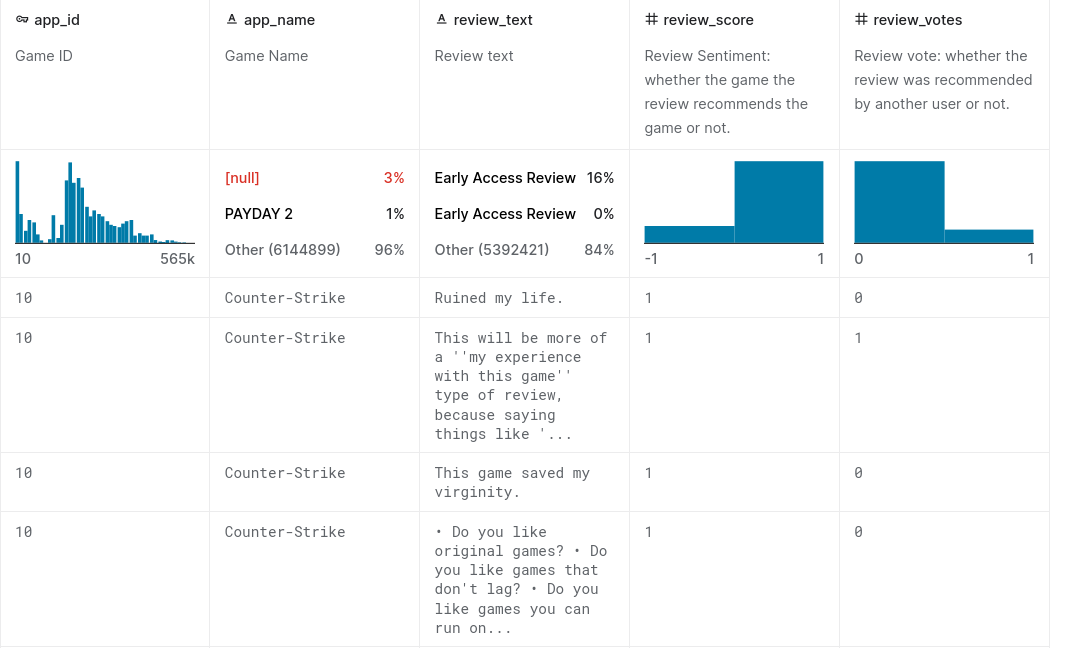
\includegraphics[width=12cm]{img/fig_1.png}
  \centering
  \caption{Steam Reviews [1]}
\end{figure}

In this project, we focus on the 'review\_text' and 'review\_score' columns to perform sentiment analysis. The 'review\_text' column provides the text data for analysis, while the 'review\_score' column serves as the sentiment label (positive if the game is recommended, negative otherwise).


\subsection{Justification}


Based on the challenges identified in the paper "Data Cleaning: Overview and Emerging Challenges" by Xu Chu and others (2016), the use of language models can potentially offer solutions to these data cleaning problems[8]. Here are some of the challenges identified in the paper and our proposed solutions using language models:

\begin{itemize}
    \item \textbf{Scalability:} Language models, when properly trained and fine-tuned, can handle data of any size and perform data cleaning tasks effectively and efficiently. This can help to scale data cleaning techniques for large and rapidly growing datasets in the Big Data era.
    
    \item \textbf{User Engagement:} With an optimized language model, the need for human intervention in data cleaning tasks can be significantly reduced. This not only increases the efficiency of the process but also mitigates the risks of human errors.
    
    \item \textbf{Semi-structured and unstructured data:} The use of machine learning tools can help detect the type of data and structure it appropriately before passing it into the cleaning model. This can help address data quality problems for semi-structured and unstructured data formats.
    
    \item \textbf{Privacy and Security Concerns:} Due to the automated nature of the data cleaning process using language models, human intervention is minimized, thereby addressing privacy and security concerns. An optimized language model doesn't require user to access the raw data, which can help to ensure privacy.
\end{itemize}

Given the challenges and findings from the above studies, we propose using language models such as GPT or T5 for data cleaning. The reasons include:

\begin{itemize}
    \item \textbf{Automation:} Language models can automate the data cleaning process, reducing manual effort and the need for exhaustive pattern matching or rule creation.
    \item \textbf{Versatility:} With the right prompt, a language model can perform various cleaning tasks, such as removing stop words, special characters, and unrelated words.
    \item \textbf{Adaptability:} Language models can keep up with evolving language use, including slangs and new semantics, by fine-tuning them on recent data.
    \item \textbf{Handling Unknowns:} Language models, especially those using attention mechanisms, can handle unknown or unexpected data elements better due to their ability to understand long-term dependencies in the data.
    \item \textbf{All-in-one tool:} With the right prompt, a language model can perform multiple cleaning tasks at once, such as removing special characters, stop words, and non-sentimental words, detecting type error and fixing them.
\end{itemize}

This approach addresses the challenges identified in the previous studies, offering a scalable, automated, and adaptable solution for data cleaning in the context of machine learning and sentiment analysis.


\subsection{Methodology}

\subsubsection{Data Processing}

The first step in our data processing pipeline involves importing our raw review data into a Pandas DataFrame for easier manipulation. We leverage a dataset of over six million Steam reviews sourced from Kaggle [1]. To make the pre-training process more manageable, we randomly select a subset of 1000 reviews, ensuring that 65\% of them are positive, and the remaining 35\% are negative. This decision was motivated by our preliminary tests that indicated significant results could be achieved with this sample size.

\begin{table}[h]
\centering
\begin{tabular}{llll}
\toprule
\textbf{Number of Reviews} & \textbf{Mean Squared Error} & \textbf{Accuracy} & \textbf{F-1 Score} \\
\midrule
1,000 & 1.08 & 73.0 & 0.791 \\
10,000 & 0.824 & 79.4 & 0.843 \\
100,000 & 0.629 & 84.285 & 0.883 \\
\bottomrule
\end{tabular}
\caption{Midterm's model performance on testing dataset of various data size using the baseline filtered review evaluated using SVM with $C=10$ as regularization parameters.}
\end{table}

\subsubsection{Creating the Baseline Reviews}

With our selected subset of 1000 reviews, we create a new column in our DataFrame named \texttt{filtered\_review\_text}. This column contains a filtered version of the raw review text, which is stored in the \texttt{review\_text} column. We also retain the sentiment labels of the original raw reviews in a column named \texttt{review\_score}.

The \texttt{filtered\_review\_text} column serves as our baseline for comparison with the reviews generated by the pre-trained language model. We generate this column using standard Python libraries, including pandas, re, nltk, and nltk.corpus.stopwords.

Our data cleaning process follows standard practices in sentiment analysis:

\begin{itemize}
    \item Conversion of reviews into lowercase to ensure uniformity and avoid duplication based on case differences.
    \item Removal of all special characters using regular expressions, reducing noise in the text data.
    \item Elimination of stopwords (commonly used words that do not contribute to the sentiment of a sentence, e.g., 'the', 'is', 'in') to focus on words that carry sentiment.
    \item Stripping trailing spaces to maintain consistency in the data.
    \item Dropping duplicate and NAs strings value review.
\end{itemize}

The result of this process is a clean and consistent set of reviews that we can use as a baseline for evaluating our language model's performance.


\subsubsection{Generating Filtered Review using Pre-trained Models}

A challenge we faced during this project was finding an accessible, capable model. Although GPT-3/4 possess impressive capabilities, they are not open source and require payment based on the number of tokens used via the API. This becomes cost-prohibitive especially with long or numerous reviews. Consequently, we decided to explore alternative models that, while not as powerful, are open source and allow for reasonable experimentation. 

We elected to use GPT-2, Google's T5, and Google's Flan [12]. Flan is an optimized fine-tuned version of the original T5 model on various NLP task, making it a genuine competitor to GPT-2 and other proprietary models. Importantly, Flan is an open-source pre-trained model, making it accessible to all for individual experimentation.

We utilized the following pre-trained models:

\begin{table}[h]
\centering
\begin{tabular}{ll}
\toprule
\textbf{Model} & \textbf{Number of Parameters} \\
\midrule
gpt2 & 117M\\
gpt2-xl & 1558M\\
t5-base & 250M\\
t5-xl & 3000M\\
flan-t5-base & 250M\\
flan-t5-xl & 3000M \\
\bottomrule
\end{tabular}
\caption{Pre-tranied models}
\end{table}

Given the computational demands of deep learning models, we used Google Colab for this project, as it provides access to powerful GPUs, which are not typically available to average individuals or on consumer-grade PCs. 

In Google Colab, we primarily used the Hugging Face transformers library to implement these models. Both the tokenizer and the pre-trained models were obtained from this source. 

For every model, the input prompt was: 

\begin{quote}
    "Keeps only sentimental words: \textit{review\_text}"
\end{quote}

We used this prompt to achieve multiple filters, such as removing special characters and non-sentimental words (i.e., stopwords, etc.). Additionally, we aimed to use fewer tokens to save on execution time. More details on run-time can be found in the results section.

The models' outputs were stored in a new column titled \texttt{model\_name}, adjacent to the original \texttt{review\_text} column.

For GPT-2, here are the parameters we used for the tokenizer and model:

\begin{verbatim}
tokenizer(input,
          max_length=50, 
          truncation=True, 
          return_tensors='tf')

model.generate(**encoded_input, 
               early_stopping=True,
               max_length=25,
               repetition_penalty = 5.2,
               top_k = 80)

tokenizer.batch_decode(output, skip_special_tokens=True)[0]
\end{verbatim}

For T5 and Flan-T5:

\begin{verbatim}
encoded_input = tokenizer(input,
                          max_length=50, 
                          truncation=True, 
                          return_tensors='pt').input_ids.to("cuda")

model.generate(encoded_input, 
               early_stopping=True,
               max_length=64)

tokenizer.batch_decode(output, skip_special_tokens=True)[0]
\end{verbatim}

Many of these parameters were chosen to save execution time.


\subsection{Validating the Filtered Review}

The objective of this project is to utilize pre-trained language models for data cleaning in sentiment analysis tasks. Consequently, our validation metric involves evaluating the performance of sentiment classification on the cleaned reviews.

To validate the effectiveness of our approach, we will compare the results of sentiment classification on the baseline filtered reviews and the cleaned reviews generated by the pre-trained models.

We will employ the same machine learning algorithms as outlined in "Exploring the Sentiment of Steam Reviews with Naive Bayes and Support Vector Machine" by Puttisan Mukneam (2023) [2]. These algorithms include Multinomial Naive Bayes with Laplacian Smoothing and Support Vector Machines (SVM) with various smoothing parameters and regularization parameters.

The performance of these algorithms will be evaluated using Mean Squared Error (MSE), Accuracy, and F1-score. These metrics will provide a comprehensive view of the model's performance, from overall accuracy to the balance between precision and recall (F1-score), and the average squared differences between predicted and actual outcomes (MSE).

In both MVB and SVM models, we drop reviews where their values were NA to combat TypeError during training and testing process. We also have split the filtered reviews. We decided to use 80\% as training data for the model, and 20\% for testing. Lastly, out of the training data, we extract 20\% to be a local testing data during the training process, in order to determine optimal parameters to be used during testing phase.

\subsubsection{Multinomial Naive Bayes}

We trained the Multinomial Naive Bayes classifier using various parameters for Laplacian smoothing. Then we evaluate model's performance on the testing data set using a fixed smoothing parameter of 0.1, and fixed the seed for reproducibility. The MultinomialNB class from the scikit-learn library was utilized for this purpose. 

\subsubsection{Linear Support Vector Machine (SVM)}

We trained a Linear Support Vector Machine (SVM) classifier with various regularization parameter C values. We also fixed the seed, and tested the model using a fixed regularization parameters of C=1. The implementation was performed using the LinearSVC function from the scikit-learn library.

\section{Result}
Here are the results and discussion of our finding.
\subsection{Testing}


\begin{table}[h]
\centering
\begin{tabular}{llll}
\toprule
\textbf{Model} & \textbf{Mean Squared Error} & \textbf{Accuracy} & \textbf{F-1 Score} \\
\midrule
Baseline & 0.7 & 82.5 & 0.865 \\
gpt2 & 1.18 & 70.5 & 0.784 \\
gpt2-xl & 1.2 & 70.0 & 0.781 \\
t5-base & 1.2 & 70.0 & 0.776 \\
t5-xl & 1.24 & 69.0 & 0.780\\
flan-t5-base & 0.96 & 75.87 & 0.821 \\
flan-t5-xl & 1.02 & 74.371 & 0.80 \\
\bottomrule
\end{tabular}
\caption{Models performance on testing dataset evaluated using SVM with $C=1$ as regularization parameters (fixed seed).}
\end{table}

\begin{table}[h]
\centering
\begin{tabular}{llll}
\toprule
\textbf{Model} & \textbf{Mean Squared Error} & \textbf{Accuracy} & \textbf{F-1 Score} \\
\midrule
Baseline & 0.74 & 81.5 & 0.864 \\
gpt2 & 1.0 & 75.0 & 0.821 \\
gpt2-xl & 1.1 & 72.5 & 0.808 \\
t5-base & 1.3 & 67.5 & 0.758 \\
t5-xl & 1.08 & 73.0 & 0.80\\
flan-t5-base & 1.25 & 74.37 & 0.815 \\
flan-t5-xl & 1.14 & 71.356 & 0.78 \\
\bottomrule
\end{tabular}
\caption{Models performance on testing dataset evaluated using Naive Bayes with $a=0.1$ as smoothing parameter (fixed seed).}
\end{table}


\subsection{Assessing Results}

The performance of the pre-trained models varied in comparison to the baseline, with both SVM and Multinomial Naive Bayes classifiers. Although the baseline model demonstrated superior performance across all metrics, the pre-trained models showed promising results despite some limitations in our experiment.

Among the pre-trained models, flan-t5-base displayed the most promising performance, with relatively low MSE, high accuracy, and a reasonably balanced F1-Score. This suggests that with the right fine-tuning and optimization, this model could potentially improve and possibly outperform traditional data cleaning methods.

The gpt2, gpt2-xl, t5-base, t5-xl, and flan-t5-xl models showed varied performance, with some performing better in certain metrics than others. While their overall performance did not exceed that of the baseline, it's essential to consider that the parameters used in this experiment were chosen to expedite run times. With more comprehensive fine-tuning, the use of optimal prompts, and a larger dataset, these models could potentially yield improved results.

It's worth noting that the size of the dataset used in this experiment was relatively small. We used only 1000 reviews, which might not fully harness the power of these models. Larger datasets could potentially provide the models with more context and variability, leading to more accurate and robust performance.

In conclusion, while the baseline model outperformed the pre-trained models in this experiment, the latter hold significant potential for improvement and application in the data cleaning domain. Future work involving optimized parameters, fine-tuning, and larger datasets could yield more promising results.

\subsection{Drawbacks of Using Pre-trained Models}

Although pre-trained models offer several advantages, there are notable drawbacks that need to be considered when implementing them for data cleaning tasks. Some of these drawbacks are as follows:

\begin{enumerate}
    \item \textbf{Computational expense:} Fine-tuning these pre-trained models is computationally expensive. It necessitates advanced resources and significant computational power, which may not be readily available to every researcher or developer. Additionally, an optimized pre-trained model for data cleaning is currently lacking, which adds to the computational overhead.


    \item \textbf{Time consumption:} Generating cleaned reviews using these models can be time-consuming.
    \begin{table}[h]
    \centering
    \begin{tabular}{ll}
    \toprule
    \textbf{Model} & \textbf{Generating time} \\
    \midrule
    gpt2 & 20m\\
    gpt2-xl & 1hr\\
    t5-base & 4m\\
    t5-xl & 25m\\
    flan-t5-base & 5m\\
    flan-t5-xl & 12m \\
    \bottomrule
    \end{tabular}
    \caption{Approximate generating time of 1000 reviews on a free Google Colab account}
    \end{table}
    
    
    
    \item \textbf{Accessibility:} Many state-of-the-art models such as GPT-3/4 are not open-source but are accessible via paid APIs. This can be prohibitive for small businesses or individual developers who cannot afford the associated costs.
    
    \item \textbf{Prompt design:} It can be challenging to design optimal prompts when the model has not been fine-tuned, as the training details of the original model may not be available or clear. This lack of transparency can lead to inefficiencies and inaccuracies in the data cleaning process.
    
    \item \textbf{Knowledge requirement:} Fine-tuning these models requires extensive knowledge and understanding of their architecture and parameters. Finding optimal parameters can be challenging and may require a large amount of data and computational resources. This again can be expensive and beyond the means of many users.

    \item \textbf{Data Bias:} Pre-trained models can carry biases from their training data. This can lead to skewed results when these models are used for data cleaning, particularly in sentiment analysis tasks.
    
    \item \textbf{Black Box Models:} Understanding why a model made a certain prediction or decision can be challenging, making it hard to diagnose issues or improve the model.
    
    \item \textbf{Lack of Flexibility:} Pre-trained models may not perfectly fit the data cleaning task at hand, requiring additional work in fine-tuning or adapting the model for the specific task.
\end{enumerate}



\section{Future Work}

Based on the challenges and limitations identified in this project, several areas of future work are suggested:

\begin{enumerate}
    \item \textbf{Fine-tuning FLAN-T5 for data cleaning:} We found that fine-tuning the FLAN-T5-base model on 300K reviews with a high-end GPU (40GB memory) and 70 compute units using Google Colab Pro took more than 9 hours. However, given the flexibility of the FLAN-T5 architecture in handling various NLP tasks, we believe it holds potential for being effectively fine-tuned to perform data cleaning tasks.
    
    \item \textbf{Exploring specialized deep learning models:} We plan to investigate more optimized deep learning models that are specifically designed for data cleaning tasks. This might help in enhancing the performance and reducing the computational overhead associated with current models.
    
    \item \textbf{Fine-tuning parameters:} There is scope for exploring different fine-tuning strategies, tokenizers, and model parameters to improve the efficacy of the pre-trained models in cleaning tasks.
    
    \item \textbf{Exploring optimal prompts:} Further work can be done to investigate and design optimal prompts for the pre-trained models to maximize their performance in data cleaning tasks.
\end{enumerate}

\section{References}

\small

[1] Sobkowicz, A. (2017). Steam Reviews Dataset. Retrieved from \url{https://www.kaggle.com/datasets/andrewmvd/steam-reviews}

[2] Mukneam, P. (2023). sentiment\_steam. Retrieved from \url{https://github.com/pmukneam/sentiment_steam}

[3] Konduru, Y. J. (2021). Game Review Classifier. Retrieved from \url{https://yaswanth3277.github.io/Portfolio/gamereviewclassifier.html}

[4] Kumar, S. (2018). IMDB movie review polarity using Naive Bayes Classifier. Retrieved from \url{https://satyam-kumar.medium.com/imdb-movie-review-polarity-using-naive-bayes-classifier-9f92c13efa2d}

[5] Reddy, V. (2018). Sentiment Analysis using SVM. Retrieved from \url{https://medium.com/@vasista/sentiment-analysis-using-svm-338d418e3ff1}

[6] Narayanan, V., Aror, I.,\& Bhatia, A. (2013). Fast and accurate sentiment classification using an enhanced Naive Bayes model. Indian Institute of Technology.

[7] Zuo, Z. (2018). Sentiment Analysis of Steam Review Datasets using Naive Bayes and Decision Tree Classifier. Retrieved from \url{http://hdl.handle.net/2142/100126}

[8] Chu, X., Ilyas, I. F., Krishnan, S., \& Wang, J. (2016). Data Cleaning: Overview and Emerging Challenges. SIGMOD’16, June 26-July 01, 2016, San Francisco, CA, USA. DOI: \url{http://dx.doi.org/10.1145/2882903.2912574}

[9] Li, P., Rao, X., Blase, J., Zhang, Y., Chu, X., \& Zhang, C. (2021). CleanML: A Study for Evaluating the Impact of Data Cleaning on ML Classification Tasks. 2021 IEEE 37th International Conference on Data Engineering (ICDE), Chania, Greece. DOI: 10.1109/ICDE51399.2021.00009.

[10] Radford, A., Wu, J., Child, R., Luan, D., Amodei, D., Sutskever, I., \& others. (2019). Language models are unsupervised multitask learners. OpenAI blog, 1(8), 9.

[11] Raffel, C., Shazeer, N., Roberts, A., Lee, K., Narang, S., Matena, M., Zhou, Y., Li, W., \& Liu, P. J. (2020). Exploring the Limits of Transfer Learning with a Unified Text-to-Text Transformer. Journal of Machine Learning Research, 21(140), 1-67.

[12] Chung, H. W., Hou, L., Longpre, S., Zoph, B., Tay, Y., Fedus, W., Li, E., Wang, X., Dehghani, M., Brahma, S., \& others. (2022). Scaling Instruction-Finetuned Language Models. arXiv. \url{https://arxiv.org/abs/2210.11416}

[13] Mukneam, P. (2023). sentiment-deep-cleaning. Retrieved from \url{https://github.com/pmukneam/sentiment-deep-cleaning}
\end{document}


